\documentclass[journal=jctcce,manuscript=article]{achemso}

\usepackage{amsmath,amssymb,mathtools}
\usepackage{booktabs}
\usepackage{siunitx}
\usepackage{tikz}

\title{Unified Atomic Synthons and BDPCS3 for Continuous Chemical Space Exploration}

\author{Vincenzo Barone}
\affiliation{Department of Chemistry, University of Bologna, Bologna, Italy}
\email{vincenzo.barone@unibo.it}

\author{Merlino Development Team}
\affiliation{Merlino Project}

\keywords{atomic synthons, continuous atom typing, BDPCS3, force-field correction, chemical space, effective atomic number}

\begin{document}

\begin{abstract}
We present a unified formulation where topology, atomic synthons, and BDPCS3 bond-length corrections share the same continuous geometric descriptors. Atomic synthons are used to define continuous atom types, explore chemical spaces, and drive geometry/force-field corrections. A key quantity is the effective atomic number, interpreted as a molecular generalization of the isolated-atom atomic number.
\end{abstract}

\section{Introduction}
Geometry-aware descriptors are central to transferable molecular models. In this framework, atomic synthons provide continuous local chemical information derived directly from Cartesian coordinates. These features serve three connected goals: continuous atom typing, exploration and organization of chemical spaces, and correction of geometry/force-field parameters.

In this work, the first correction target is BDPCS3: only bond lengths are corrected from DPCS3 because angles and dihedrals are already sufficiently accurate in routine use.

\paragraph{Central concept: effective atomic number.}
The effective atomic number is the continuous molecular extension of atomic number:
\begin{equation}
Z^{\mathrm{eff}}_i = Z_i-\frac{1}{2}+\mathrm{EAN}_i,
\end{equation}
where $\mathrm{EAN}_i$ is a normalized synthon magnitude (bounded in $[0,1)$). Writing
\begin{equation}
\mathbf{s}_i=
\left(
\operatorname{erf}\!\left(\frac{q_i}{\sigma_{\mathrm{EAN}}}\right),
\operatorname{erf}\!\left(\frac{C_i}{\sigma_{\mathrm{EAN}}}\right),
\operatorname{erf}\!\left(\frac{D_i}{\sigma_{\mathrm{EAN}}}\right),
\operatorname{erf}\!\left(\frac{S_i}{\sigma_{\mathrm{EAN}}}\right)
\right),
\qquad
\mathrm{EAN}_i=\frac{\lVert\mathbf{s}_i\rVert_2}{1+\lVert\mathbf{s}_i\rVert_2},
\end{equation}
it is explicit that $Z_i^{\mathrm{eff}}$ is atomic number plus a normalized synthon norm correction (with the constant shift $-0.5$).

\section{Methods}
\subsection{Descriptor construction}
Starting from Cartesian coordinates, we compute continuous coordination numbers, coordination-dependent covalent radii, and topology bond orders. Atomic synthons are then built from the same quantities, giving one consistent descriptor layer.

\subsection{BDPCS3 coupling}
BDPCS3 corrections are applied to DPCS3 bond lengths using topology-consistent bond orders:
\begin{equation}
\mathrm{BO}_{ij}^{\mathrm{BDPCS3}} \leftarrow \mathrm{BO}_{ij}^{\mathrm{topo}}.
\end{equation}

\section{Results and Discussion}
The unified design enforces consistency: topology computes continuous coordination and bond order, synthons use the same definitions, and BDPCS3 uses topology-consistent bond order. This removes descriptor drift across modules and improves interpretability.

\section{Compact Equation Summary}
Updated BDPCS3 parameters are:
\begin{equation}
K=6.0\times10^{-3},\qquad
\Delta r=0.17~\text{\AA},\qquad
\sigma=0.057~\text{\AA}.
\end{equation}
CH amplification appears as $1+0.25\,\chi_{\mathrm{CH},ij}$, with $\chi_{\mathrm{CH},ij}=\delta_{Z_i,6}\delta_{Z_j,1}+\delta_{Z_i,1}\delta_{Z_j,6}$.

\section{Conclusions}
Atomic synthons provide a unified feature layer for atom typing, chemical-space exploration, and geometric correction. BDPCS3 is the first operational example where synthon-consistent bond order (and coordination context) corrects DPCS3 bond lengths while keeping already accurate geometric components unchanged.

\section*{Data and Code Availability}
All equations and implementation details correspond to the Merlino 3.0 repository modules for topology, synthons, and BDPCS3 workflows.

\begin{acknowledgement}
The authors acknowledge the Merlino development environment and all contributors who supported testing and validation of the topology and BDPCS3 workflows.
\end{acknowledgement}

\begin{suppinfo}
Supplementary Information includes: additional numerical comparisons between legacy and updated BDPCS3 corrections; descriptor-level examples for representative chemical motifs; and implementation notes for reproducibility.
\end{suppinfo}

\appendix
\section{Complete Equation Set (Unabridged)}

\subsection{Continuous topology layer}
Given Cartesian geometry $\{\mathbf{R}_i\}$ and atomic numbers $\{Z_i\}$:
\begin{equation}
\mathrm{CNA}_i = \sum_{j\neq i} g_{ij},
\qquad
g_{ij} = \frac{1}{2}\left[1+\operatorname{erf}\!\left(\alpha_{\mathrm{CNA}}\,(R^0_{ij}-R_{ij})\right)\right],
\end{equation}
with
\begin{equation}
R_{ij}=\lVert \mathbf{R}_i-\mathbf{R}_j\rVert,
\qquad
R^0_{ij}=R^{\mathrm{cov}}(Z_i)+R^{\mathrm{cov}}(Z_j).
\end{equation}

\begin{equation}
\tilde R^{\mathrm{cov}}_i = \mathcal{H}\!\left(Z_i,\mathrm{CNA}_i\right),
\end{equation}
where $\mathcal{H}$ is a $C^1$ Hermite interpolation between tabulated Pyykko coordination radii.

\begin{equation}
\mathrm{BO}_{ij}^{\mathrm{topo}}
=\exp\!\left(
\frac{\tilde R^{\mathrm{cov}}_i+\tilde R^{\mathrm{cov}}_j-R_{ij}}{\lambda_{\mathrm{BO}}}
\right).
\end{equation}

\subsection{Atomic synthons}
\begin{align}
N_{\pi,i} &= \sum_{j\in\mathcal{N}(i)} \max(\mathrm{BO}_{ij}-1,0),\\
N_{\mathrm{res},i} &= n^{\mathrm{val}}_i-\mathrm{CNA}_i-N_{\pi,i},\\
N_{\mathrm{OS},i} &= \mathrm{mod}\!\left(\mathrm{round}(N_{\mathrm{res},i}),2\right),\\
N_{\mathrm{LP},i} &= \max\!\left(0,\frac{N_{\mathrm{res},i}-N_{\mathrm{OS},i}}{2}\right),\\
N_{\mathrm{ED},i} &= \mathrm{CNA}_i+N_{\mathrm{LP},i}+N_{\mathrm{OS},i}.
\end{align}

\begin{align}
q_i &= \sum_{j\in\mathcal{N}(i)}
\frac{\chi_j-\chi_i}{(n_i+n_j)\,\max(\mathrm{BO}_{ij},\mathrm{BO}_{\min})},\\
C_i &= \frac{1}{|\mathcal{N}(i)|}\sum_{j\in\mathcal{N}(i)}
\frac{\tilde R^{\mathrm{cov}}_i+\tilde R^{\mathrm{cov}}_j}
{R_{ij}+\tilde R^{\mathrm{cov}}_i+\tilde R^{\mathrm{cov}}_j},\\
D_i &= \frac{1}{|\mathcal{N}(i)|\,\bar R_i}\sum_{j\in\mathcal{N}(i)}\left|R_{ij}-\bar R_i\right|,
\quad
\bar R_i=\frac{1}{|\mathcal{N}(i)|}\sum_{j\in\mathcal{N}(i)}R_{ij},\\
\mathrm{EAN}_i &= \frac{\sqrt{\sum_{k=1}^{4}\left[\operatorname{erf}(x_{k,i}/\sigma_{\mathrm{EAN}})\right]^2}}
{1+\sqrt{\sum_{k=1}^{4}\left[\operatorname{erf}(x_{k,i}/\sigma_{\mathrm{EAN}})\right]^2}},
\end{align}
with $x_{k,i}\in\{q_i,C_i,D_i,S_i\}$.

\begin{equation}
Z^{\mathrm{eff}}_i = Z_i-\frac{1}{2}+\mathrm{EAN}_i.
\end{equation}

\begin{equation}
\Sigma_i=\left(Z_i,\ \mathrm{aromatic}_i,\ \mathrm{round}(N_{\mathrm{ED},i}),\ \mathrm{round}(\mathrm{CNA}_i)\right).
\end{equation}

\subsection{Updated BDPCS3}
\begin{equation}
r_{ij}^{\mathrm{BDPCS3}} = r_{ij}^{\mathrm{DPCS3}}+\Delta r_{ij},
\end{equation}
\begin{equation}
\Delta r_{ij}
=A_{ij}(r_{ij})
\left[1-\chi_{\mathrm{CS}}(i)\chi_{\mathrm{CS}}(j)
\exp\!\left(-\left(\frac{r_{ij}-r^{\mathrm{cov}}_{ij}+\Delta r}{\sigma}\right)^2\right)\right],
\end{equation}
with
\begin{equation}
A_{ij}(r)
=-K\,r^{\mathrm{cov}}_{ij}
\left(1+0.25\,\chi_{\mathrm{CH},ij}\right)
\left[\max(n_i,n_j)^2-1\right]
f_{\mathrm{coord}}(r),
\end{equation}
\begin{equation}
f_{\mathrm{coord}}(r)=\frac{1}{2}\left[1-\operatorname{erf}\!\left(\frac{r-(r^{\mathrm{cov}}_{ij}+0.35)}{\sigma}\right)\right].
\end{equation}

\begin{align}
\chi_{\mathrm{CS}}(x)&=\delta_{Z_x,6}+0.5\,\delta_{Z_x,16},\\
\chi_{\mathrm{CH}}(x)&=\delta_{Z_x,6}+\delta_{Z_x,1}.
\end{align}

\begin{equation}
K=6.0\times10^{-3},\qquad
\Delta r=0.17~\text{\AA},\qquad
\sigma=0.057~\text{\AA}.
\end{equation}

\paragraph{Implementation form.}
\begin{equation}
\Delta r_{ij}
=\left[-K\,r^{\mathrm{cov}}_{ij}(1+0.25\,\chi_{\mathrm{CH},ij})N_{ij}f_{\mathrm{coord}}(r)\right]
\left(1-\chi_{\mathrm{CS},ij}e^{-((r-r^{\mathrm{cov}}_{ij}+\Delta r)/\sigma)^2}\right),
\end{equation}
with $\chi_{\mathrm{CH},ij}=\chi_{\mathrm{CH}}(i)\chi_{\mathrm{CH}}(j)$,
$\chi_{\mathrm{CS},ij}=\chi_{\mathrm{CS}}(i)\chi_{\mathrm{CS}}(j)$,
$N_{ij}=\max(n_i,n_j)^2-1$.

\subsection{Legacy BDPCS3 (reference)}
\begin{align}
\Delta r^{\mathrm{legacy}}_{ij} &= \Delta b^{\mathrm{CV}}_{ij}+\Delta b^{\mathrm{V}}_{ij},\\
\Delta b^{\mathrm{CV}}_{ij}
&= -0.0011\left(1+1.1\,\delta_{\mathrm{CH}}\right)\sqrt{n_i n_j-1}\;r^{\mathrm{cov}}_{ij},\\
\Delta b^{\mathrm{V}}_{ij}
&= \Delta b^{\mathrm{CV}}_{ij}\left(\sqrt{|\mathrm{BO}_{ij}-2|}-1\right)
\quad\text{(selected pairs)},
\end{align}
with weak-bond damping:
\begin{equation}
\mathrm{if}\ \mathrm{BO}_{ij}<0.3,\quad \Delta r^{\mathrm{legacy}}_{ij}=0.
\end{equation}

\begin{tocentry}
\centering
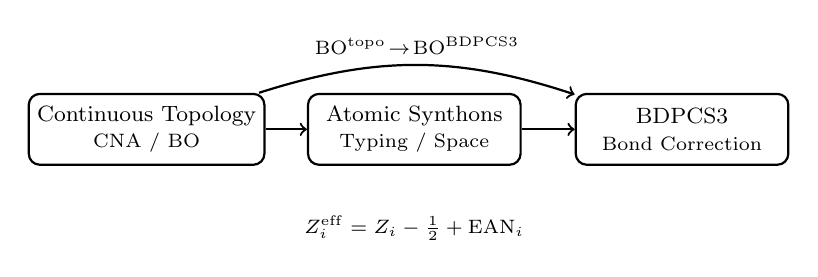
\begin{tikzpicture}[x=1cm,y=1cm,baseline=(current bounding box.center)]
\tikzstyle{box}=[draw,rounded corners,thick,align=center,inner sep=3pt,font=\footnotesize]
\node[box,minimum width=2.7cm,minimum height=0.9cm] (topo) at (0,0) {Continuous Topology\\\scriptsize CNA / BO};
\node[box,minimum width=2.7cm,minimum height=0.9cm] (syn) at (3.4,0) {Atomic Synthons\\\scriptsize Typing / Space};
\node[box,minimum width=2.7cm,minimum height=0.9cm] (bdp) at (6.8,0) {BDPCS3\\\scriptsize Bond Correction};

\draw[->,thick] (topo) -- (syn);
\draw[->,thick] (syn) -- (bdp);
\draw[->,thick] (topo) to[bend left=18] node[above,font=\scriptsize] {$\mathrm{BO}^{\mathrm{topo}}\!\to\!\mathrm{BO}^{\mathrm{BDPCS3}}$} (bdp);

\node[align=center,font=\scriptsize] at (3.4,-1.25) {$Z_i^{\mathrm{eff}}=Z_i-\frac{1}{2}+\mathrm{EAN}_i$};
\end{tikzpicture}
\end{tocentry}

\end{document}
